\documentclass{article}[13pt]
\usepackage[spanish]{babel}
\usepackage[utf8]{inputenc}
\usepackage{geometry}
 \geometry{
 a4paper,
 total={170mm,257mm},
 left=20mm,
 top=20mm,
 }
 \usepackage{graphicx}
 \usepackage{titling}

 \usepackage{fancyhdr}
 \fancypagestyle{plain}{%  the preset of fancyhdr 
     \fancyhf{} % clear all header and footer fields
     \fancyfoot[R]{}
     \fancyfoot[L]{\thedate}
     \fancyhead[L]{Introducción a la Investigación Experimental}
     \fancyhead[R]{\theauthor}
 }
\setlength{\headheight}{13pt}
 \makeatletter
 \def\@maketitle{%
   \newpage
   \null
   \vskip 1em%
   \begin{center}%
   \let \footnote \thanks
     {\LARGE \@title \par}%
     \vskip 1em%
     %{\large \@date}%
   \end{center}%
   \par
   \vskip 1em}
 \makeatother
 
 \usepackage{lipsum}  
 \usepackage{cmbright}
\title{Estudio de la Difusión en Función de la Variación de Temperatura}
\author{Andrés Felipe Pinzón Harker}
\date{\today}

\begin{document}
\maketitle

\noindent\begin{tabular}{@{}ll}
    Estudiante & \theauthor\\
    Profesor & Fabio Enrique Fajardo Tolosa
\end{tabular}
%-----------------------------------------
\section*{Objetivos}
\begin{enumerate}
    \item Verificar la constante de difusividad de diferentes sustancias (tinta) a partir de la Teoría de Einstein para el movimiento browniano con variaciones de temperatura.
    \item Verificar la ley de Fick para Difusividad respecto el tiempo y el espacio en dos dimensiones.
\end{enumerate}
%-----------------------------------------
\section*{Marco Teórico}
La \textbf{difusión} es el transporte de materia de un punto a otro mediante el movimiento térmico de átomos o moléculas~\cite{mehrerHistoryBibliographyDiffusion2007} impulsadas a través de la interacción por los gradientes de concentración descritos empíricamente en primer lugar por las \textbf{leyes de Fick}~\cite{gilExperimentosFisicaUsando2014}. La difusión es un fenómeno físico termodinámico gobernado por interacciones mecánico cuánticas atribuidas de la Teoría de Einstein sobre el movimiento browniano~\cite{einsteinUberMolekularkinetischenTheorie1905} que justifican la dinámica de la ley de Fick, es responsable de la mezcla de gases, líquidos y solidos de manera espontanea sin que ocurra un movimiento macroscópico del sistema como lo puede ser la convección, el medio se homogeneizará en un estado donde la densidad de concentración de la sustancia en ese medio tenderá a disminuir en el espacio y el tiempo~\cite{gilExperimentosFisicaUsando2014}.

La primera ley de Fick~\cite{gilExperimentosFisicaUsando2014} relaciona los flujos de partículas por unidad de área $\mathbf{J}$ y los gradientes de concentración $\nabla \mathbf{n}$ en la ec. \ref{eq:fick1}:
\begin{equation}
    \mathbf{J} = -D \nabla \mathbf{n},
    \label{eq:fick1}
\end{equation}
donde $n\equiv n(x,y,z;t)$ es la concentración del soluto, generalmente cantidad en mol o número de partículas por unidad de volumen; $\mathbf{J}\equiv\mathbf{J}(t)$ es el flujo de partículas o moles por unidad de área; y por último $D$ es el coeficiente de \textit{difusividad} que en general dependerá de distintas condiciones  detalladas por la Teoría de Einstein-Stokes.
La segunda ley de Fick es descrita a partir de la ecuación de continuidad del fluido en un elemento infinitesimal de volumen $\Delta V$ que relaciona el flujo del material respecto el tiempo a partir de la ec.~\ref{eq:fick1.5}
\begin{equation}
    \nabla \mathbf{J} = -\frac{\partial n}{\partial t},
    \label{eq:fick1.5}
\end{equation}
% sería bueno determinar teóricamente este valor.
que da forma a la difusión o segunda ley de Fick en ec.~\ref{eq:fick2}
\begin{equation}
    \frac{\partial n}{\partial t} = D \nabla^2 n.
    \label{eq:fick2}
\end{equation}

Es esencial destacar la aportación de la Teoría de Einstein-Stokes~\cite{einsteinUberMolekularkinetischenTheorie1905} que relaciona el coeficiente de difusividad $D$ con la temperatura $T$ y el radio de la partícula $r$ en la ec. \ref{eq:einstein} para la suposición de movimiento browniano en un fluido newtoniano a temperatura constante en un medio isótropo~\cite{leeInkDifussionWater2004}
\begin{equation}
    D = \frac{k_B T}{6 \pi \eta r},
    \label{eq:einstein}
\end{equation}
donde $k_B$ es la constante de Boltzmann, $\eta$ es la viscosidad del medio y $a$ el tamaño de pequeñas esferas en el medio viscoso. La ec. \ref{eq:einstein} describe el movimiento browniano de una partícula en un fluido, donde el coeficiente de difusividad $D$ es inversamente proporcional a la viscosidad del medio y directamente proporcional a la temperatura.

Aplicando la ecuación de Fick a un medio bidimensional, la solución de la ecuación diferencial parcial por método de separación de variables~\cite{gilExperimentosFisicaUsando2014} queda descrita en La ec. \ref{eq:fick2d}
\begin{equation}
    n(r,t) = \frac{A_0}{2 D t} \exp{\left\{-\frac{r^2}{4Dt}\right\}},
    \label{eq:fick2d}
\end{equation}
donde $N$ es el número de partículas iniciales, $r$ es el radio euclidiano $r^2 = x^2 + y^2$ sobre las coordenadas del espacio, $t$ es el tiempo y $D$ es el coeficiente de difusividad. 
%-----------------------------------------
\section*{Descripción del Experimento}
El arreglo experimental se basa en casi su totalidad en Salvador Gil con el esquema propuesto como en la fig. \ref{fig:esquema_experimental}
\begin{figure}[htp]
    \centering
    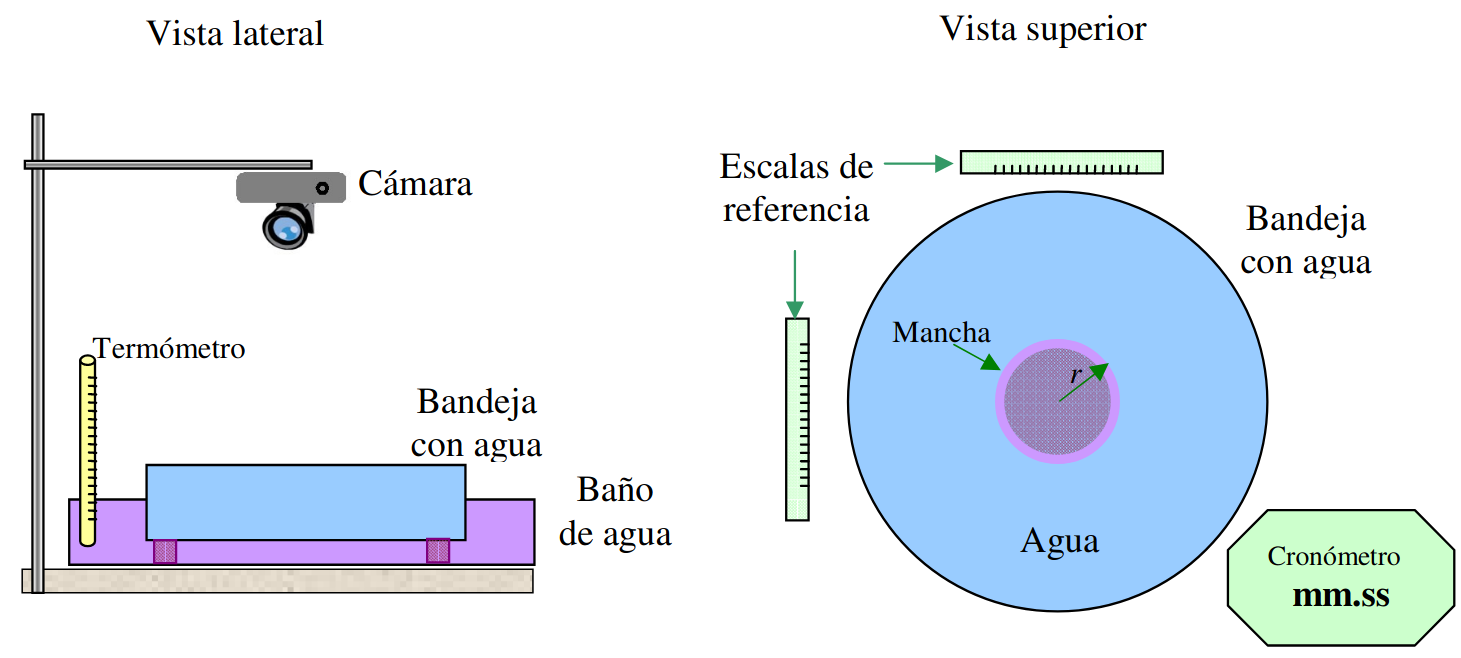
\includegraphics[width=0.8\textwidth]{figs/esquema_refGil.png}
    \caption{Esquema del experimento de difusión en dos dimensiones. Tomado de~\cite{gilExperimentosFisicaUsando2014}.}
    \label{fig:esquema_experimental}
\end{figure}
Se dispone un recipiente de vidrio con agua destilada sobre un baño de agua termalizada a una temperatura $T_a$ en base a una resistencia $R$ que varíe la temperatura. Las escalas de referencia en vertical y horizontal como reglas milimetradas ($\Delta r = \pm 0.1 cm$), aunque también se puede disponer de una grilla como un papel milimetrado, aunque las condiciones de visibilidad pueden no ser efectivas. Se utilizará un cronómetro de referencia ($\Delta t = \pm 0.1 \, \unit{\second}$) que será leído por la cámara posicionada en un soporte en posición cenital al fenómeno, se utilizará un cuentagotas con tinta  \textit{Quink blue ink} puesta en el punto central del recipiente y si es posible para líquido-líquido, mientras que el permanganato de Potasio (KMnO$_4$) como referencia solida-líquido.

Se espera que el material se difunda en el agua, se tome un video y se pueda estudiar bajo el software \texttt{tracker} y software de análisis de imagenes como \texttt{ImageJ (Fiji)}, se estudiarán las variables de radio $r\pm\Delta r$ respecto tiempo $t\pm\Delta t$, se repetirá con distintas temperaturas $T$.
%-.-.-.-.-.-.-.-.-.-.-.-.-.-.-.-.-.-.-.-.-.-.-.-.-.-.-.-.
\subsection*{Variables Físicas}
Las variables principales que \textbf{no controlo} son:
\begin{itemize}
    \item \textbf{Concentración} $\mathbf{n}$ (mol/cm$^3$): Se espera que el fabricante determine la concentración de la tinta inicial $\mathbf{n}_0$ y en el tiempo y el espacio es un parámetro dependiente, luego se tomará el perfil de luminancia para determinarlo.
    \item \textbf{Difusividad} $\mathbf{D}$ (m$^2$/s): Se espera que el coeficiente de difusividad de la tinta en agua sea determinado por las condiciones según ec. \ref{eq:einstein}, aunque hay una derivación teórica utilizando la energía de activación química~\cite{leeInkDifussionWater2004}.
    \item \textbf{Temperatura ambiental} $\mathbf{T_a}$ (K): Se esperan condiciones no demasiado variables para que nuestro baño de agua termalice correctamente el recipiente con agua puesto que no tenemos inserto el termómetro directamente para condiciones ideales homogéneas. Se tendrá que determinar un error mayor a partir de esta apreciación.
    \item \textbf{Pureza del agua} $\mathbf{C}$ (mol/cm$^3$): Si no se consigue agua destilada o esta es de mala calidad, los minerales e impurezas generarán un medio inhomogéneo.
    \item \textbf{Resolución de la cámara} $\mathbf{\Delta r}$ (cm): Debido al presupuesto y la estabilidad del video no es una condición controlable, luego la incertidumbre del radio podrá variar, aunque puede reducirse con una cámara mejor y de fotografía ``continua''.
    \item \textbf{Viscosidad} $\mathbf{\eta}$ ($\unit{\pascal} \cdot \unit{\second}$): Podremos controlar parcialmente la viscosidad de la tinta según la viscosidad inicial (¿determinada por fabricante?).
    \item \textbf{Radio} $\mathbf{r}$ (cm): El radio de difusión será medido a partir de las imágenes obtenidas del experimento, utilizando software de análisis de imágenes.
\end{itemize}

Las variables principales que \textbf{controlaré} son las siguientes, teniendo en cuenta que aquella con (S) serán sistemáticas:
\begin{itemize}
    \item[(S)] \textbf{Temperatura del Baño} $T_b$ (K): Se espera que la temperatura del agua pueda variarse y termalizarse con la temperatura real $T$ del recipiente, que se pueda variar entre $T_b = 10 \pm 1 \, \unit{\degreeCelsius}$ y $T_b = 40 \pm 1 \, \unit{\degreeCelsius}$ para evitar perturbaciones por evaporación u otros. Se espera tener curvas diferentes curvas de difusión para cada temperatura y posterior hacer el análisis en el rango lineal\cite{leeInkDifussionWater2004}.
    \item[(S)] \textbf{Tiempo} $t$ (s): Se espera medir rangos de tiempo suficientemente largos para verificar el fenómeno completo basado en $\tau\equiv Dt$ tiempos de difusión con cronómetro. Se tienen también curvas de $\tau$ respecto cada $n$ vs $t$ \cite{leeInkDifussionWater2004}.
    \item[(S)] \textbf{Cantidad} $m$ (gr): Se espera que la cantidad de tinta sea controlada por el cuentagotas que tendrá determinado un peso a partir de la densidad de la tinta $\rho_0$ o medición directa. La variación de la masa no está clara, pero se espera que influya en el radio máximo $r_{\text{max}}$ de forma lineal.
    \item \textbf{Radio máximo} $r_{\text{max}}$ (cm): Se tiene control de las medidas de los envases según un posible tanteo o previa revisión de las condiciones geométricas del experimento.
\end{itemize}
%-----------------------------------------
\section*{Materiales}
Los materiales variarán dependiendo del presupuesto y disponibilidad, se categorizan como esenciales (E), preferibles (P) y opcionales (O):
\begin{itemize}
    \item[(E)] \textbf{Recipiente Baño}: Recipiente con baja conductividad térmica, de vidrio o plástico, con un aislamiento extra en la base.
    \item[(E)] \textbf{Recipiente Principal}: Recipiente con alta conductividad térmica para reducir los tiempos de termalización del agua respecto al baño, pueda ser de aluminio u otro material.
    \item[(E)] \textbf{Agua destilada y normal}: Agua destilada de fácil compra y referencia.
    \item[(E)] \textbf{Cámara}: Cámara de video con alta resolución, dependiente de la busqueda de un buen equipo.
    \item[(E)] \textbf{Resistencia Térmica}: Resistencia de cerámica capaz de calentar el agua a temperaturas hasta 40°C y posiblemente más de manera estable.
    \item[(E)] \textbf{Termómetro}: Termómetro de alta precisión, posiblemente digital o termistor calibrado para tener seguridad en fluctuaciones de temperatura para establecer una correcta propagación.
    \item[(E)] \textbf{Cronómetro}: Cronómetro digital de precisión.
    \item[(E)] \textbf{Reglas}: Reglas milimetradas o papel milimetrado para establecer la escala de referencia.
    \item[(E)] \textbf{Soporte}: Estable y ajustable en tres grados de libertad.
    \item[(P o E)] \textbf{Tinta \textit{Quink blue ink}}: Tinta de alta calidad, posiblemente de la marca \textit{Parker} o similar para buena referencia, sino tinta china.
    \item[(P)] \textbf{Permanganato de Potasio}: KMnO$_4$ como referencia de difusión sólida-líquido con alto contraste.
    \item[(O)] \textbf{Cámara 2}: Cámara para toma de video o fotografía que acompaña a la cámara principal y hace lo alterno.
    \item[(O)] \textbf{Cuentagotas}: Donde se pueda medir lo que se implementa.
    \item[(O)] \textbf{Celda Peltier}: Para controlar la temperatura del agua de manera más precisa, aunque no es necesario.
    \item[(O)] \textbf{Iluminación}: Luz LED o fluorescente para mejorar la calidad de la imagen y el contraste para determinar la concentración de difusión $n$.
\end{itemize}
%-----------------------------------------
\section*{A resolver}
A título personal, con este experimento, me gustaría entender los fenómenos de difusión en materiales por condiciones microscópicas, a un ideal de extender esta forma de flujo a partículas en un medio nuclear, donde se ha visto el flujo de la misma manera pero con condiciones de un potencial. En ese sentido, me gustaría resolver el proceso a partir de la mecánica estadística a el fenómeno termodinámico \cite{reif2009fundamentals}.

También, me gustaría conocer más en detalle cuando se perturba el medio, porque el ideal también está lejos de lo que podemos ver en fenomenos de difusión en la realidad, luego a partir de vibraciones mecánicas, de un medio inhomogeneo, con geometría irregular o con fenómenos de dinámicos.

%-----------------------------------------
\section*{Bibliografía}
La referencia principal del trabajo experimental se basa en el libro de Salvador Gil~\cite{gilExperimentosFisicaUsando2014}, que genera tres diferentes casos de estudio experimental. Referencias teóricas como `Diffsion in Solids' \cite{mehrerHistoryBibliographyDiffusion2007}, Mecánica de Fluidos de Cengel~\cite{çengel2006mecánica}, completan el marco fundamental para la comprensión de la difusión y el movimiento browniano. Se referencia clásicamente el trabajo original de Einstein~\cite{einsteinUberMolekularkinetischenTheorie1905} y Fick \cite{fickLiquidDiffusion1995}, y además como extensión al proceso experimental se incluye el trabajo de Lee~\cite{leeInkDifussionWater2004} que describe la difusión de tinta en agua. Como referencias auxiliares para procesos teóricos más extensos y aproximados a condiciones no ideales se encuentran lo estudios de Bringuier et. al.~\cite{Bringuier_2009} que describen la difusión en procesos de no equilibrio, la aportación química, tipos de difusión termodinámica y fenómenos de transporte, y Glicksman et. al.~\cite{didomizioSimulationFicksVerification2006} con verificaciones a partir de simulaciones computacionales.

\bibliographystyle{IEEEtran}
\bibliography{references}
\end{document}
